\documentclass{report}[12pt]
\usepackage[margin=2cm]{geometry} % Set the margins to 2.5cm on all sides
\usepackage{lipsum} % For generating "Lorem Ipsum" text
\usepackage{fancyhdr} % For custom headers
\usepackage[hidelinks]{hyperref} % For hyperlinks
\usepackage{graphicx} % For including images
\usepackage{svg} % For including SVG images
\usepackage{relsize} % For resizing text
\usepackage{titlesec} % For customizing chapter titles
\usepackage{titletoc} % For customizing the table of contents
\usepackage{scalefnt} % For scaling fonts
\usepackage[document]{ragged2e}
\usepackage{setspace} % For customizing line spacing

\usepackage{listings}
\usepackage{xcolor}
% Modern font setup
\usepackage{fontspec}
\usepackage{pdfpages}
\setmainfont{Roboto}


\definecolor{codegreen}{rgb}{0,0.6,0}
\definecolor{codegray}{rgb}{0.5,0.5,0.5}
\definecolor{codepurple}{rgb}{0.58,0,0.82}
\definecolor{backcolour}{rgb}{0.95,0.95,0.92}

\lstdefinestyle{mystyle}{
    backgroundcolor=\color{backcolour},   
    commentstyle=\color{codegreen},
    keywordstyle=\color{magenta},
    numberstyle=\tiny\color{codegray},
    stringstyle=\color{codepurple},
    basicstyle=\ttfamily\footnotesize,
    breakatwhitespace=false,         
    breaklines=true,                 
    captionpos=b,                    
    keepspaces=true,                 
    numbers=left,                    
    numbersep=5pt,                  
    showspaces=false,                
    showstringspaces=false,
    showtabs=false,                  
    tabsize=2
}

% Title and author information
\title{\Huge\textbf{Ensuring Ethical Compliance in DevOps Implementation for Regulated Industries}}
\author{\Large Neelanjan Mukherji}

% % Header setup
% \pagestyle{fancy}
% \fancyhf{} % Clear existing header/footer settings
% \fancyhead[R]{\nouppercase{\leftmark}} % Display chapter name (without chapter number) on the right side of the header
% \fancyfoot[R]{\thepage} % Display page number on the right side of the footer
% \renewcommand{\headrulewidth}{0.4pt} % Add horizontal line below the header


% Header setup
\pagestyle{fancy}
\fancyhf{} % Clear existing header/footer settings
\fancyhead[R]{\nouppercase{\leftmark}} % Display chapter name (without chapter number) on the right side of the header
\fancyfoot[R]{\thepage} % Display page number on the right side of the footer
\renewcommand{\headrulewidth}{0.4pt} % Add horizontal line below the header


\begin{document}

% Title page
\begin{titlepage}
    \centering
    
\includegraphics[width=0.4\textwidth]{./Assets/Amity-Logo-Solo}\par
    % \includesvg{./Assets/Amity-Logo-Solo}\par
    \vspace*{0.1cm}
    {\scshape\Huge \textbf{Non-Teaching Credit Course(NTCC)} \par}
    {\scshape\Huge \textbf{Term Paper/Report[ETTP100]} \par}
    {\scshape\LARGE Amity Unversity Greater Noida \par}
    \vspace*{1cm}
    {\LARGE Topic : \par}
    \vspace*{0.3cm}
    {\Huge\textbf{Ensuring Ethical Compliance in DevOps Implementation for Regulated Industries}}\par
    \vspace{1cm}
    {\Large Supervisor:}\par

    {\Large \textbf{Mr. Bhanu Prakash Lohani \& Mr. Pradeep Kumar Kushwaha}}\par
    {\Large Department of Computer Science And Engineering}\par
    \vspace{1cm}
    {\Large Submitted by:}\par
    % \vspace{0.2cm}
    {\Large \textbf{Neelanjan Mukherji}}\par
    {\Large A41105221002}\par
    \vspace{1cm}
    {\Large B.Tech. (Computer Science Engineering)}\par
    {\Large \textbf{Semester - V}}\par
    % \vfill
    % {\Large Date: \today}\par
\end{titlepage}

\tableofcontents

% Abstract
\chapter*{Abstract}
\addcontentsline{toc}{chapter}{Abstract}
\justifying
\paragraph{\textbf{Background:}}
\paragraph{\textbf{Aim:}} 
\paragraph{\textbf{Method:}} 
\paragraph{\textbf{Results:}} 
\paragraph{\textbf{Conclusion:}}  % Abstract text is in a separate file for easier

% Certificate
\chapter*{Certificate}
\addcontentsline{toc}{chapter}{Certificate}
\input{Certificate/certificate.tex} % Certificate text is in a separate file for easier

% Declaration of Submission
\chapter*{Declaration of Submission}
\addcontentsline{toc}{chapter}{Declaration of Submission}

% Acknowledgement
\chapter*{Acknowledgement}
\addcontentsline{toc}{chapter}{Acknowledgement}
I would like to express my gratitude to...

% Plagiarism Certificate
\chapter*{Plagiarism Certificate}
\addcontentsline{toc}{chapter}{Plagiarism Certificate}

I hereby declare that the content of this report is original and does not infringe upon the intellectual property rights of any third party.


% Chapters
\chapter*{Executive Summary}
\addcontentsline{toc}{chapter}{Executive Summary}

Executive Summary:

This report focuses on the crucial aspect of ensuring ethical compliance in DevOps implementation for regulated industries. DevOps practices, characterized by their collaborative, automated, and continuous delivery approach, have gained significant traction in sectors such as healthcare, finance, and pharmaceuticals. However, implementing DevOps in these industries poses unique ethical challenges that must be addressed to maintain compliance and uphold ethical standards.

The objective of this report is to provide organizations operating in regulated industries with a comprehensive understanding of the ethical considerations surrounding DevOps implementation. By exploring the regulatory framework and compliance standards specific to these sectors, organizations can navigate the complex landscape and ensure adherence to legal and regulatory requirements.

The report delves into the ethical issues associated with DevOps practices, including data privacy and protection, security and vulnerability management, transparency, accountability, and regulatory compliance. These considerations are essential for organizations to build and maintain trust with stakeholders, safeguard sensitive information, and meet regulatory obligations.

To establish an ethical DevOps culture, the report emphasizes the importance of leadership and governance, ethical decision-making frameworks, training and awareness programs, and the establishment of a code of ethics and conduct. It further explores specific DevOps practices that promote ethics, such as secure software development, continuous integration and delivery, infrastructure as code, and automation and orchestration.

In addition to organizational practices, the report addresses the ethical considerations involved in selecting appropriate DevOps tools and vendors. Evaluating toolchain options based on ethical criteria and assessing vendors for their ethics and compliance practices are essential steps in mitigating ethical risks during the implementation process.

The report also presents case studies of ethical DevOps implementations in regulated industries, providing real-world examples of successful approaches. Furthermore, it proposes an ethical compliance assessment framework to help organizations evaluate their compliance posture and identify areas for improvement.

By adhering to the recommendations outlined in this report, organizations can ensure ethical compliance in their DevOps implementations, foster a culture of responsibility and accountability, and uphold the trust of customers, regulators, and other stakeholders. Ultimately, by embedding ethical considerations into DevOps practices, regulated industries can achieve successful and compliant digital transformation while maintaining ethical integrity.

% \begin{enumerate}

% \item Executive Summary
%    \item Introduction
%       The executive summary provides an overview of the report's focus on ensuring ethical compliance in DevOps implementation for regulated industries. It highlights the growing importance of DevOps practices in regulated sectors and acknowledges the ethical challenges that arise in this context.
   
%     \item Objective of the Report
%       The objective of the report is to examine the ethical considerations associated with DevOps implementation in regulated industries and to provide actionable recommendations for organizations to establish and maintain ethical DevOps practices. By doing so, it aims to promote responsible and compliant use of DevOps methodologies within the regulatory framework.

%     \item Key Findings
%       This section summarizes the key findings derived from the research and analysis conducted for the report. It highlights the ethical challenges specific to DevOps implementation in regulated industries and identifies crucial areas of focus for organizations seeking to ensure ethical compliance.

%     \item Recommendations
%       The recommendations section offers practical guidance and best practices for organizations to effectively address ethical challenges in DevOps implementation. It covers areas such as leadership and governance, ethical decision-making frameworks, training and awareness programs, and the establishment of a code of ethics and conduct. The recommendations also emphasize the need for secure software development practices, compliance assessment frameworks, and responsible toolchain selection.
% \end{enumerate}

\chapter{Background}

\section*{Introduction}
\paragraph{In order to grasp the full extent of the report, we will delve into the fundamentals and explore the foundational aspects of DevOps.}

\paragraph{DevOps serves as a conceptual framework aimed at reconciling the development and operations aspects of Information Systems. Its primary objective is to dismantle barriers between developers and operations professionals. By implementing a set of principles and practices, DevOps enhances work processes, emphasizing the importance of seamless collaboration between development and operations teams.\cite{diel2016communication}}

\paragraph{Having explored the fundamental concepts and principles of DevOps, we now shift our focus to an integral component of its implementation: Version Control Systems (VCS). In today's fast-paced software development landscape, where collaboration and continuous integration are paramount, VCS plays a crucial role in ensuring seamless coordination, efficient code management, and reliable version tracking. This section delves into the significance of VCS within the DevOps framework, examining its functionalities, benefits, and the popular tools used in the industry. By understanding the pivotal role of version control in enabling successful DevOps practices, we can appreciate its impact on streamlining development processes and fostering a culture of agility and innovation.}

\section*{Version Control Systems}

Version Control Systems (VCS) help developers manage their source codes and keep track of every version of their projects. It is a tool that allows for efficient organization, coordination, and collaboration among software developers, enabling them to work together towards creating improved projects. VCS plays a crucial role in Software Engineering by facilitating teamwork and ensuring a smooth development process.\cite{zolkifli2018version}

\subsection*{Types of Version Control Systems}

There are primarily two types of version control systems: centralized version control systems (CVCS) and distributed version control systems (DVCS).

\subsubsection*{Centralized Version Control Systems (CVCS)}
CVCS stores the complete history of a project in a central repository, which serves as a single point of truth. Users access files from the central server, make changes, and commit them. Popular CVCS examples include Concurrent Versions System (CVS) and Apache Subversion (SVN).

\subsubsection*{Distributed Version Control Systems (DVCS)}
DVCS provides a distributed architecture where each user maintains a local copy of the entire project, including the full history. Users can work offline, commit changes locally, and synchronize with other repositories as needed. Git, Mercurial, and Bazaar are prominent examples of DVCS.

\newpage

\subsection*{Key Functionalities}

VCS offer several key functionalities that benefit software development and collaborative projects:

\subsubsection*{Versioning and History}
VCS enables the creation of a versioned history of files and directories, capturing changes over time. This allows users to view and revert to previous versions, providing a safety net and facilitating easy bug tracking.

\subsubsection*{Branching and Merging}
Branching allows for the creation of parallel development lines, enabling developers to work on new features or bug fixes without affecting the main codebase. Merging integrates changes from one branch into another, ensuring smooth collaboration and code integration.

\subsubsection*{Collaboration and Conflict Resolution}
VCS enables multiple users to work concurrently on the same project, handling conflicts that arise when two or more users make conflicting changes to the same file. It provides tools for conflict resolution, ensuring efficient collaboration and minimizing code conflicts.

\subsubsection*{Tagging and Labeling}
VCS allows developers to tag specific versions, marking them as significant milestones or releases. Tags serve as references for stable versions and facilitate reproducibility and software release management.

\subsection*{Benefits of Version Control Systems}

Implementing a version control system provides numerous benefits for software development teams and collaborative projects:

\subsubsection*{Change Tracking and Accountability}
VCS logs every change made to files, enabling teams to track who made the changes and when. This promotes accountability and facilitates auditing and debugging processes.

\subsubsection*{Collaboration and Concurrent Development}
VCS enables multiple developers to work simultaneously on the same project, ensuring seamless collaboration and avoiding conflicts through branching and merging mechanisms.

\subsubsection*{Code Stability and Recovery}
By maintaining a complete history of changes, VCS allows teams to revert to previous versions in case of code issues, ensuring code stability and quick recovery from errors.

\subsubsection*{Experimentation and Feature Development}
Version control systems facilitate experimentation by allowing developers to create new branches and try out different features or approaches without impacting the main codebase. This promotes innovation and flexibility in development.

\subsubsection*{Documentation and Knowledge Sharing}
VCS provides a documented record of changes, making it easier to understand the evolution of a project. It also serves as a knowledge-sharing platform, allowing developers to learn from past decisions and experiences.

\newpage

\subsection*{Popular Version Control System Tools}

There are several widely used version control system tools available, each with its unique features and advantages:

\subsubsection*{Git}
Git is a distributed version control system known for its speed, scalability, and branching capabilities. It is widely adopted in the software development community and offers extensive support and a rich ecosystem of third-party tools.

\subsubsection*{Subversion (SVN)}
Subversion is a centralized version control system that offers a user-friendly interface and seamless integration with existing workflows. It provides robust versioning and collaboration features, suitable for both small and large projects.

\subsubsection*{Mercurial}
Mercurial is a distributed version control system designed for ease of use and scalability. It emphasizes simplicity and straightforwardness while offering powerful branching and merging capabilities.

\subsubsection*{Perforce}
Perforce is a centralized version control system widely used in enterprise settings. It provides excellent performance, scalability, and security features, making it suitable for large-scale projects and organizations.

\subsection*{Application of VCS}

\subsubsection*{Code Integration}

\begin{enumerate}
    \item Code integration is a fundamental process in Version Control Systems (VCS) that involves merging changes from one branch or code repository into another. It facilitates the seamless combination of different code changes, allowing developers to incorporate their modifications into a common codebase. This process ensures collaboration, synchronization, and the overall stability of software development projects. In this section, we will delve into the concept of code integration in VCS, its importance, and the steps involved in the process.
    \item \textbf{Understanding Code Integration : }Code integration is a crucial aspect of collaborative software development, especially in scenarios where multiple developers are working on the same project concurrently. When developers work on separate branches or local copies of the codebase, code integration allows them to consolidate their changes, resolve conflicts, and merge their modifications into a shared branch or repository. The main goals of code integration are to synchronize changes, maintain a coherent codebase, and ensure the stability and functionality of the software.
    \item \textbf{Importance of Code Integration : } Effective code integration offers several benefits for software development projects:
    \begin{enumerate}
        \item Collaboration: Code integration enables multiple developers to work on different aspects of a project simultaneously. It promotes collaboration by allowing developers to share their changes and combine their efforts, fostering a more efficient and productive development process.
        \item Consistency: Integration ensures that all modifications are combined in a controlled manner, maintaining the consistency and integrity of the codebase. It helps prevent inconsistencies and conflicts that can arise when developers work independently and allows for a cohesive software product.
        \item Bug Detection: Code integration facilitates the detection of bugs or issues that may arise due to incompatible changes. By merging and testing code changes together, developers can identify and resolve conflicts, inconsistencies, and potential bugs early in the development cycle.
        \item Stable Releases: By integrating changes from different branches, developers can create stable releases that incorporate new features, bug fixes, and improvements. This process ensures that the released software is reliable and functional, meeting the requirements and expectations of end-users.
    \end{enumerate}
    \item \textbf{Steps Involved in Code Integration : }The code integration process typically involves the following steps:
    \begin{enumerate}
        \item Selecting the Source and Target: The first step is to identify the source branch or repository containing the changes that need to be integrated. The target branch or repository is where the changes will be merged into.
        \item Resolving Conflicts: Conflicts may arise when there are overlapping modifications in the source and target branches. Developers need to review and resolve these conflicts by analyzing the conflicting code and making appropriate adjustments to ensure compatibility and consistency.
        \item Performing the Integration: Once conflicts are resolved, the changes from the source branch are merged into the target branch. The VCS system applies the necessary modifications to the target branch, incorporating the new code while preserving existing code and functionality.
        \item Testing and Verification: After integration, thorough testing is crucial to ensure the stability and functionality of the integrated code. Developers perform various tests, including unit tests, integration tests, and system tests, to verify that the merged code functions as intended and does not introduce new issues.
        \item Review and Feedback: Code integration may involve a review process, where other team members or stakeholders examine the integrated code and provide feedback. This helps ensure code quality, adherence to coding standards, and the overall improvement of the software.
    \end{enumerate}
    \item \textbf{VCS Tools for Code Integration : }Popular VCS tools provide specific features and workflows to facilitate code integration. For example:
    \begin{enumerate}
        \item Git: Git offers powerful branching and merging capabilities, making it a widely used VCS tool for code integration. It provides commands such as `git merge` and `git rebase` to integrate changes from one branch into another, along with options for conflict resolution.
        \item Subversion (SVN): SVN also supports code integration through commands like `svn merge` and provides mechanisms to handle conflicts and manage the integration process.

        \item Mercurial: Mercurial includes features for merging and integrating changes between branches. It offers commands such as `hg merge` and provides tools to resolve conflicts during the integration process.
    \end{enumerate}
    \item Code integration is a crucial aspect of collaborative software development using Version Control Systems. It enables multiple developers to merge their changes into a common codebase, fostering collaboration, consistency, and stable software releases. By following the steps involved in the integration process and utilizing VCS tools with robust merging capabilities, development teams can ensure efficient and successful code integration, leading to high-quality software products.
\end{enumerate}



\subsubsection*{Collaborative Workflow}

\begin{enumerate}
    \item Collaborative workflow refers to the process and practices employed in software development teams to enable efficient collaboration using Version Control Systems (VCS). It involves utilizing VCS features and strategies to facilitate seamless teamwork, effective communication, and coordinated development efforts. In this section, we will explore the concept of collaborative workflow in VCS, its benefits, and the key elements involved.
    \item \textbf{Understanding Collaborative Workflow : }Collaborative workflow in VCS encompasses the methodologies, practices, and tools used by development teams to work together on a shared codebase. It leverages the capabilities of VCS to enable concurrent development, code sharing, code review, and coordination among team members. By utilizing a collaborative workflow, teams can enhance productivity, maintain code quality, and streamline the software development process.
    \item \textbf{Key Elements of Collaborative Workflow : }A collaborative workflow in VCS typically involves the following key elements:
    \begin{enumerate}
        \item Branching and Merging: Branching allows team members to work on separate branches of the codebase, enabling parallel development of different features or bug fixes. Merging brings these branches together, combining the changes into a shared branch, ensuring code integration, and resolving any conflicts that may arise.
        \item Code Sharing and Collaboration: VCS provides mechanisms for sharing code changes, allowing developers to exchange modifications, review each other's code, and provide feedback. Collaborative features such as pull requests or code reviews enable effective collaboration, knowledge sharing, and improved code quality.
        \item Conflict Resolution: Collaborative workflow requires efficient conflict resolution mechanisms. Conflicts occur when multiple developers modify the same portion of code simultaneously. VCS tools provide features to identify conflicts and support the resolution process, ensuring that code changes can be merged seamlessly.
        \item Communication and Coordination: Effective communication is essential in a collaborative workflow. VCS tools often provide features such as comments, notifications, and task tracking, allowing team members to communicate, discuss code changes, assign tasks, and coordinate their efforts.
        \item Continuous Integration (CI) and Automated Testing: Collaborative workflows often integrate with CI systems, which automatically build and test the codebase. CI ensures that code changes from different team members are integrated and tested frequently, detecting issues early and providing rapid feedback.
    \end{enumerate}
    \item \textbf{Benefits of Collaborative Workflow : }Implementing a collaborative workflow in VCS offers several advantages:
    \begin{enumerate}
        \item Improved Team Productivity: Collaborative workflows foster effective teamwork, enabling developers to work in parallel, share knowledge, and leverage each other's expertise. This leads to increased productivity and faster development cycles.
        \item Code Quality and Review: Collaborative workflows encourage code reviews and collaboration between team members. Code reviews help identify bugs, improve code quality, maintain coding standards, and promote knowledge sharing within the team.
        \item Version Control and History: Collaborative workflows leverage the version control capabilities of VCS, ensuring a complete history of code changes. This allows teams to understand the evolution of the codebase, revert to previous versions if needed, and maintain a comprehensive audit trail.
        \item Agile Development and Iterative Processes: Collaborative workflows align well with agile development methodologies. Teams can work on user stories or features independently, integrating changes frequently, and adapting to evolving requirements. This enables iterative development and quick feedback loops.
        \item Reduced Conflicts and Code Duplication: Collaborative workflows, including proper branching and merging strategies, help reduce conflicts and code duplication. By segregating work into branches, developers can work on isolated features or bug fixes, minimizing interference with other team members' code.
    \end{enumerate}
    \item \textbf{VCS Tools for Collaborative Workflow : }Various VCS tools offer features and integrations to support collaborative workflows:
    \begin{enumerate}
        \item Git: Git is a widely used VCS with strong support for collaborative workflows. It provides branching, merging, and code review features through pull requests, making it popular for collaborative development.
        \item Subversion (SVN): SVN also offers collaborative features, including branching, merging, and repository-level access control. It allows teams to coordinate their development efforts effectively.
        \item Mercurial: Mercurial provides capabilities for collaborative workflows, including branching, merging, and code sharing. It emphasizes simplicity and ease of use while facilitating effective collaboration.
    \end{enumerate}
    \item A collaborative workflow in VCS enables software development teams to work together efficiently, leverage each other's skills, and coordinate their efforts seamlessly. By utilizing VCS features for branching, merging, code sharing, and conflict resolution, teams can enhance productivity, code quality, and collaboration. Embracing a collaborative workflow leads to better software development outcomes and promotes effective teamwork in the context of version control systems.
\end{enumerate}

\subsubsection*{Code modifications/Code revisions}
\begin{enumerate}
    \item Code modifications or code revisions refer to the changes made to the source code of a software project within a Version Control System (VCS). VCS tracks and manages these modifications, providing a detailed history of code changes over time. In this section, we will explore the concept of code modifications in VCS, their significance, and how VCS tools facilitate managing and tracking these revisions.
    \item \textbf{Understanding Code Modifications/Revisions : }Code modifications or revisions encompass any changes made to the source code of a software project. They can range from minor edits, bug fixes, and enhancements to major feature implementations or architectural refactoring. VCS provides mechanisms to capture and store these modifications, allowing developers to track, review, and manage the evolution of the codebase.
    \item \textbf{Significance of Code Modifications/Revisions : }Code modifications within VCS offer several benefits and serve crucial purposes:
    \begin{enumerate}
        \item History and Auditing: VCS records each code modification, capturing details such as the author, timestamp, and specific changes made. This historical information provides an audit trail, allowing developers to trace back and understand the progression of the codebase. It helps in identifying the introduction of bugs or issues and supports troubleshooting and debugging processes.
        \item Collaboration and Teamwork: VCS enables multiple developers to work on the same codebase concurrently. Code modifications are tracked individually, allowing developers to collaborate effectively, share changes, and merge their modifications without conflicts. It promotes teamwork and facilitates seamless coordination among team members.
        \item Versioning and Rollbacks: Code modifications in VCS facilitate versioning, enabling developers to create snapshots of the codebase at different points in time. This allows for easy rollbacks to previous versions if new changes introduce regressions or unforeseen issues. It provides a safety net and supports stable software releases.
        \item Code Review and Quality Assurance: VCS allows code modifications to be reviewed by team members. Code review processes help identify and address potential issues, maintain coding standards, and improve overall code quality. By providing a systematic and structured approach to reviewing changes, VCS supports robust quality assurance practices.
    \end{enumerate}
    \item \textbf{Managing Code Modifications/Revisions in VCS : }VCS tools offer a range of features and workflows to effectively manage code modifications:
    \begin{enumerate}
        \item Committing Changes: Developers use VCS commands to commit their code modifications into the repository. A commit captures a snapshot of the changes made, along with associated metadata such as the author, timestamp, and commit message. This process stores the modifications and makes them available for other team members.
        \item Branching and Merging: VCS allows developers to create branches, enabling parallel development. Branches provide isolated environments for making modifications without affecting the main codebase. After completing the modifications, developers merge their branches back into the main branch, incorporating the changes into the codebase.
        \item Conflict Resolution: When multiple developers modify the same file or code section simultaneously, conflicts can arise during the merging process. VCS tools provide mechanisms to identify and resolve these conflicts, ensuring that modifications are combined seamlessly.
        \item Annotating and Annotating Tools: VCS tools often provide annotation or blame features that display the author and revision details for each line of code. This helps identify who made specific modifications, aiding in understanding the context and reasoning behind the changes.
        \item Diffing and Comparing: VCS tools enable developers to compare different versions of files or the entire codebase, highlighting the specific modifications made. Diffing features help understand the differences between revisions, supporting code review, and aiding in troubleshooting.
    \end{enumerate}
    \item \textbf{Popular VCS Tools for Managing Code Modifications/Revisions : }Several VCS tools offer robust features for managing code modifications:
    \begin{enumerate}
        \item Git: Git is a distributed VCS that excels in managing code modifications. It provides a powerful set of commands for committing, branching, merging, and tracking changes, making it a popular choice for version control.

        \item Subversion (SVN): SVN is a centralized VCS that offers comprehensive features for managing code modifications. It provides versioning, branching, and merging capabilities, allowing teams to effectively track and collaborate on code changes.

        \item Mercurial: Mercurial is a distributed VCS that facilitates managing code modifications through its intuitive interface and powerful revision control features. It offers functionalities such as branching, merging, and history tracking.
    \end{enumerate}
    \item Code modifications or revisions in VCS play a vital role in software development, providing a mechanism to track, manage, and collaborate on changes made to the codebase. They support collaboration, versioning, code review, and quality assurance processes. VCS tools enable developers to commit changes, create branches, resolve conflicts, and annotate code, ensuring efficient management of code modifications throughout the development lifecycle.
\end{enumerate}

\subsubsection*{Branching}

\begin{enumerate}
    \item Branching is a fundamental concept in Version Control Systems (VCS) that enables developers to create independent lines of development within a software project. It allows multiple versions of the codebase to exist concurrently, facilitating parallel work, experimentation, and isolation of changes. In this section, we will explore the concept of branching in VCS, its significance, and the benefits it provides to software development teams.
    \item \textbf{Understanding Branching : }Branching involves creating a separate line of development within a VCS, diverging from the main codebase or a particular branch. Each branch represents a unique version of the code, allowing developers to work independently on different features, bug fixes, or experiments without interfering with the main codebase. Branches can be created, modified, merged, and deleted as needed, providing flexibility and control over the development process.
    \item \textbf{Significance of Branching : }Branching in VCS offers several benefits and serves crucial purposes:
    \begin{enumerate}
        \item Parallel Development: Branching allows multiple developers to work on different features or bug fixes simultaneously. Each developer can create their own branch, enabling independent work without conflicts or disruptions. This parallel development improves productivity and accelerates the development process.

        \item Isolation of Changes: Branches provide an isolated environment for making changes. Developers can experiment, implement new features, or refactor code without affecting the stability or functionality of the main codebase. If a change does not meet expectations or introduces issues, it can be discarded or modified without impacting other team members' work.

        \item Risk Mitigation: Branching mitigates the risk associated with introducing new features or making significant modifications. By working on separate branches, developers can thoroughly test and validate their changes before merging them into the main codebase. This minimizes the impact of potential issues on the stability of the overall system.

        \item Release Management: Branching plays a vital role in managing software releases. Stable branches can be created to represent specific releases or versions of the software. These branches allow for bug fixes and maintenance while development continues on other branches. It provides a stable foundation for maintaining older versions while new features are being developed.

        \item Collaboration and Code Review: Branching supports collaboration and code review processes. Developers can share their branches with teammates for feedback, review, and collaboration. Branch-based workflows, such as pull requests, allow team members to discuss, review, and provide feedback on code changes before merging them into the main codebase.
    \end{enumerate}
    \item \textbf{Branching Strategies : }Various branching strategies exist, depending on the specific needs and workflows of a development team:
    \begin{enumerate}
        \item Feature Branching: Developers create branches dedicated to working on specific features. Each branch focuses on a single feature or user story, allowing independent development and easy tracking of progress. Once the feature is complete, the branch is merged back into the main codebase.

       \item Release Branching: Release branches are created to prepare a stable version of the software for deployment. These branches are used for bug fixes, maintenance, and preparing the release while development continues on other branches. Once the release is ready, it can be merged into the main codebase or a long-term maintenance branch.

        \item Hotfix Branching: Hotfix branches are created to address critical issues or bugs found in the production environment. These branches allow for swift fixes without disrupting ongoing development. Once the fix is complete, the branch is merged into the appropriate branches, including both the main codebase and other active branches.

        \item Experimental Branching: Experimental branches are used for testing new ideas, implementing risky changes, or conducting experiments without affecting the stability of the main codebase. Developers can freely experiment and iterate within these branches, either discarding or merging the changes as appropriate.
    \end{enumerate}
    \item \textbf{Managing Branches in VCS : }VCS tools provide mechanisms for creating, managing, and merging branches:
    \begin{enumerate}
        \item Creation: Developers can create branches using VCS commands or tools. The branch is typically created from an existing branch, such as the main codebase or another branch, and given a unique name to represent its purpose.

        \item Modification: Developers work on their branches, making modifications, implementing features, or fixing bugs. They can commit changes to their branch independently, ensuring that modifications are tracked and recorded.

        \item Merging: Once the work on a branch is complete, developers merge their branch back into the main codebase or another target branch. Merging combines the changes made in the branch with the target branch, ensuring the integration of new features, bug fixes, or other modifications.

        \item Conflict Resolution: During the merging process, conflicts may arise when changes overlap or conflict with each other. VCS tools provide mechanisms to identify and resolve these conflicts, allowing developers to choose how to reconcile the conflicting changes.

        \item Branch Deletion: After a branch has served its purpose and its changes have been successfully merged, it can be deleted. This helps maintain a clean and manageable branch structure, reducing clutter and complexity.
    \end{enumerate}
    \item Branching is a powerful feature of Version Control Systems that enables parallel development, isolation of changes, risk mitigation, collaboration, and effective release management. By leveraging branching strategies and utilizing VCS tools' capabilities, development teams can work concurrently on different features, experiment without affecting stability, and maintain control over the development process. Branching enhances productivity, promotes collaboration, and facilitates efficient software development within the context of Version Control Systems.
\end{enumerate}

Now that we have explored the concept of version control systems in detail, let's shift our gears and dive into the world of Git, one of the most widely used and powerful VCS tools available today.

\newpage
\section*{Git}

Git is a distributed version control system (VCS) that revolutionized the way software projects are managed and collaborated upon. It was created by Linus Torvalds in 2005 to address the scalability and performance limitations of existing VCS tools. In this report, we will delve into the world of Git, examining its key features, benefits, and its impact on modern software development practices.

\subsection*{Key Features of Git}

\begin{enumerate}
    \item Distributed Architecture: Unlike centralized VCS, Git follows a distributed model where each user has a complete local copy of the repository. This allows for offline work, faster operations, and increased resilience.

    \item Branching and Merging: Git's powerful branching and merging capabilities enable parallel development, easy experimentation, and seamless integration of changes. Developers can create branches, work on features independently, and merge their changes back into the main codebase.

    \item Lightweight and Fast: Git is designed to be lightweight, with a small footprint and fast performance. It achieves this through efficient data storage, compression techniques, and optimized algorithms, allowing for swift operations even on large codebases.

    \item Commit History and Tracking: Git provides a detailed commit history, capturing the evolution of the codebase over time. Developers can easily track changes, view commit metadata, and understand the context behind modifications.

    \item Staging Area: Git introduces the concept of a staging area or index, where developers can selectively choose which changes to include in a commit. This granular control allows for more flexible and organized commits.

    \item Distributed Collaboration: Git facilitates seamless collaboration among distributed teams. Developers can share their changes through repositories, clone remote repositories, and synchronize modifications using push and pull operations.
\end{enumerate}

\subsection*{Benefits of Git}
\begin{enumerate}
    \item Scalability: Git's distributed architecture makes it highly scalable, allowing projects of any size to be efficiently managed. The system handles large codebases with ease, making it suitable for both small teams and large enterprise projects.
    \item Speed and Performance: Git's optimized design ensures fast operations, even on complex codebases with extensive histories. This enables developers to work efficiently, reducing wait times and increasing productivity.
    \item Flexibility and Branching Strategies: Git's branching and merging capabilities provide unparalleled flexibility in managing concurrent development efforts. It supports various branching strategies, such as feature branching or release branching, enabling teams to tailor their workflows to project requirements.
    \item Versioning and Rollbacks: Git's version control capabilities allow for easy versioning and rollbacks. Developers can tag specific points in the codebase, create branches for different releases, and revert to previous versions if needed, providing a safety net during software development.
    \item Collaboration and Code Review: Git's distributed nature and support for remote repositories facilitate efficient collaboration. Developers can clone repositories, work on separate branches, review and discuss changes through pull requests, and integrate modifications seamlessly.
\end{enumerate}

\subsection*{Git in Modern Software Development}
\begin{enumerate}
    \item Open Source and Community: Git has gained immense popularity and has become the de facto standard for version control in open-source projects. It has a thriving community, with extensive documentation, online resources, and support from developers worldwide.
    \item Integration and Ecosystem: Git integrates with various development tools, such as integrated development environments (IDEs), continuous integration/continuous delivery (CI/CD) systems, and code review platforms. This integration strengthens the software development ecosystem and streamlines workflows.
    \item Adoption and Industry Impact: Git has had a significant impact on the software development industry, transforming the way teams collaborate, manage code, and track changes. Its popularity and widespread adoption have made it an essential skill for developers and a standard requirement in many software development job roles.
\end{enumerate}

\subsection*{Applications of Git}
Git, as a versatile and widely adopted version control system, finds extensive applications across various areas of software development. Its robust features, distributed architecture, and collaborative capabilities make it a valuable tool for teams of all sizes. In this section, we will explore the diverse applications of Git and how it benefits different aspects of the software development lifecycle.

\begin{enumerate}
    \item \textbf{Source Code Management : }Git's primary application lies in source code management, enabling teams to track, manage, and version their codebase effectively. It offers the following benefits:
    \begin{enumerate}
        \item Version Control: Git tracks changes at a granular level, providing a detailed history of modifications. This enables developers to easily navigate through different versions, review changes, and revert to previous states when needed.
        \item Collaboration: Git allows multiple developers to work on the same codebase concurrently. It enables seamless collaboration by providing mechanisms to merge and synchronize changes, resolve conflicts, and review code through pull requests.
        \item Branching and Parallel Development: Git's branching and merging capabilities facilitate parallel development, where developers can work on separate branches to implement features, bug fixes, or experiments. Branches provide isolation, allowing changes to be developed independently and merged back into the main codebase.
        \item Code Review: Git integrates with code review tools and workflows, enabling teams to perform thorough code reviews. It allows developers to submit changes for review, comment on code, suggest improvements, and ensure code quality before merging it into the main codebase.
    \end{enumerate}
    \item \textbf{Continuous Integration and Deployment (CI/CD) : }Git plays a vital role in CI/CD workflows, ensuring smooth and automated software delivery. Its applications in this area include:
    \begin{enumerate}
        \item Integration with CI/CD Tools: Git seamlessly integrates with CI/CD tools, enabling automated build, test, and deployment processes. CI/CD pipelines can be triggered by code changes, and Git repositories serve as the source of truth for these pipelines.
        \item Automated Testing: Git's versioning capabilities support the creation of automated test suites. Tests can be executed against different versions or branches, ensuring that changes do not introduce regressions and maintaining code quality.
        \item Continuous Deployment: Git, combined with CI/CD practices, allows for continuous deployment of software. It enables automated deployment pipelines that deliver new features or bug fixes to production environments efficiently and reliably.
    \end{enumerate}
    \item \textbf{Project Management and Collaboration : }Git facilitates project management and collaboration, enhancing team productivity and coordination. Its applications in this domain include:
    \begin{enumerate}
        \item 3.1 Task Tracking: Git integrates with project management tools that enable teams to link code changes to specific tasks, issues, or user stories. This helps in tracking progress, associating changes with their corresponding requirements, and maintaining traceability.

        \item Team Collaboration: Git's distributed nature and support for remote repositories enable geographically distributed teams to collaborate effectively. Developers can work on their local copies, share changes through repositories, and synchronize modifications using push and pull operations.

        \item Workflow Customization: Git's flexibility allows teams to define and customize their workflows. They can adopt various branching strategies (e.g., feature branching or GitFlow) and tailor their processes to meet their project's specific needs and requirements.
    \end{enumerate}
    \item \textbf{Open-Source Development : }Git has become the go-to version control system for open-source development, powering numerous collaborative projects. Its applications in the open-source ecosystem include:
    \begin{enumerate}
        \item Code Contribution: Git simplifies the process of contributing code to open-source projects. Developers can fork repositories, make changes in their own branches, and submit pull requests to have their changes reviewed and potentially merged into the main codebase.
        \item Community Collaboration: Git's distributed nature fosters community collaboration and enables developers from around the world to contribute to open-source projects. It facilitates code review, feedback exchange, and knowledge sharing within the open-source community.
        \item Project Forking and Branching: Git allows individuals or teams to create forks of existing projects. Forking enables independent development, experimentation, and customization while maintaining the project's original source as a base. Developers can also create branches within forks to work on specific features or improvements.
    \end{enumerate}
    \item \textbf{Documentation and Content Management : } Git is not limited to code but can also be used for managing documentation, content, and other non-code assets. Its applications in this area include:
    \begin{enumerate}
        \item Versioning and Tracking: Git's version control capabilities extend beyond code, making it suitable for managing documentation, configuration files, and other project assets. It enables tracking changes, reviewing modifications, and maintaining a history of content revisions.

        \item Collaboration: Git's collaborative features facilitate teamwork in documentation and content creation. Multiple contributors can work on different branches, review and comment on changes, and merge updates to create a cohesive and up-to-date final product.

        \item Content Publishing: Git can be used for publishing content, such as websites or documentation sites, by leveraging Git-based publishing platforms. It allows for easy deployment of changes, ensuring that published content reflects the latest updates from the Git repository.
    \end{enumerate}
    \item Git's versatility and powerful features make it indispensable in various applications within the software development lifecycle. From source code management to collaboration, CI/CD workflows, project management, open-source development, and content management, Git provides the foundation for efficient and collaborative software development. Its distributed architecture, branching capabilities, and seamless integration with development tools have positioned Git as a standard and widely adopted version control system in the industry.
\end{enumerate}


Git has revolutionized the world of version control systems with its distributed architecture, powerful branching capabilities, speed, and flexibility. Its benefits, such as scalability, collaboration support, and efficient code management, have made it a cornerstone of modern software development practices. Git's impact on the industry and its widespread adoption underline its significance in empowering developers to work effectively, collaborate seamlessly, and manage codebase versions with ease.

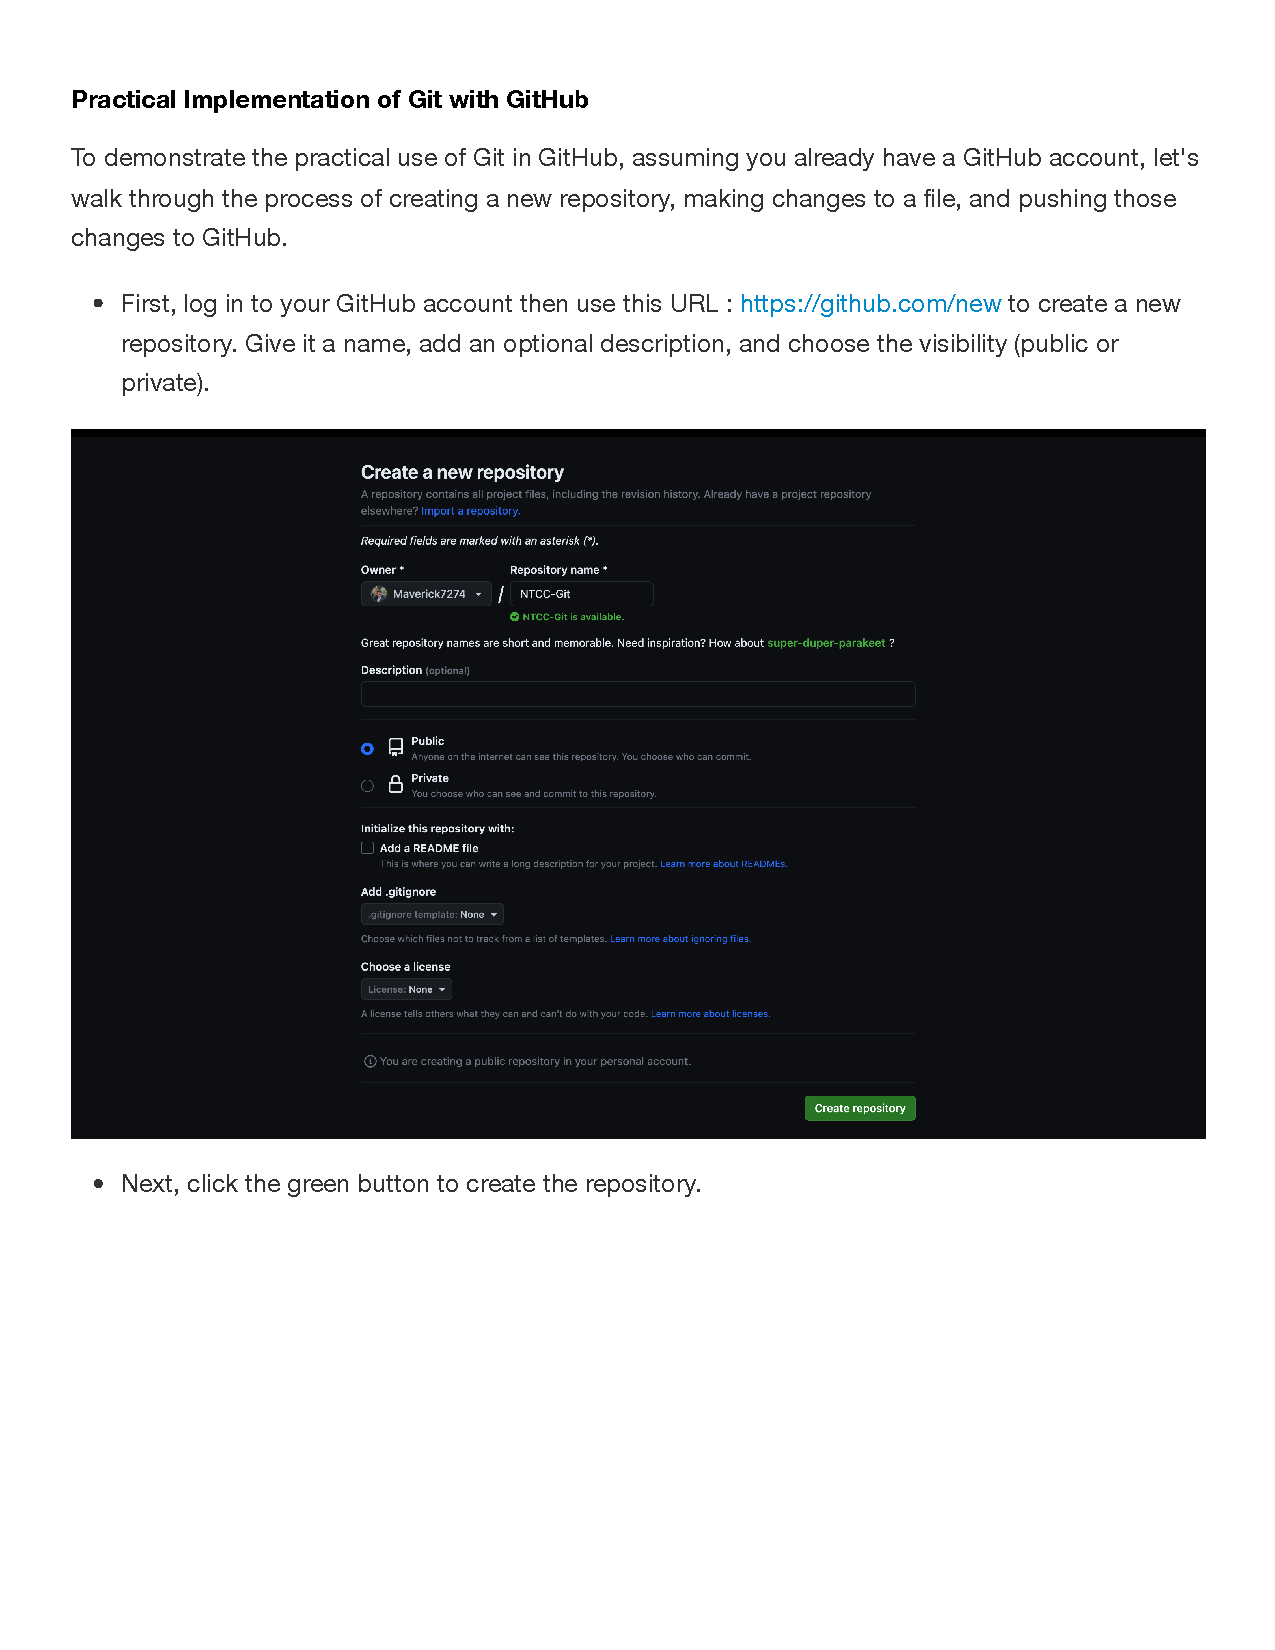
\includepdf[pages=-]{Assets/git.pdf}

After grasping the fundamentals of Git, we can now dive into the world of Containers, a powerful technology that enables the creation, deployment, and management of lightweight and portable software environments.

\section*{Containers}

\begin{enumerate}
    \item Containers are a revolutionary technology that allows you to package an application and its dependencies into a single, portable unit. These self-contained units, known as containers, provide a consistent and isolated runtime environment for applications, irrespective of the underlying operating system or infrastructure.

    \item At the core of containers is the containerization engine, the most popular of which is Docker. Docker allows you to define and build containers using a simple, declarative syntax called Dockerfile. This file specifies the base image, dependencies, and instructions for setting up the application environment. With Docker, you can easily create, distribute, and run containers on any system that supports Docker, providing a consistent and reproducible environment across different development and deployment stages.

    \item One of the key advantages of containers is their lightweight nature. Containers leverage the host operating system's kernel and share resources with other containers, resulting in efficient resource utilization and reduced overhead compared to traditional virtual machines. Containers start quickly and can be scaled up or down rapidly to meet demand, making them highly efficient for both development and production environments.

    \item Containers also promote the concept of immutable infrastructure. Once a container is built, it becomes an immutable artifact that can be versioned, tested, and deployed consistently across different environments. This approach ensures that the application behaves consistently, regardless of the deployment target.

    \item Furthermore, containers foster a modular and microservices-oriented architecture. By breaking down an application into smaller, loosely coupled components, each running within its own container, you can achieve greater scalability, maintainability, and ease of deployment. Containers enable the seamless orchestration of these microservices, allowing you to manage complex application ecosystems efficiently.

    \item Containerization also promotes a DevOps-friendly culture by facilitating collaboration between developers and operations teams. Containers provide a standardized environment for developers to package their applications and their dependencies, ensuring that they work reliably across different deployment environments. Operations teams benefit from simplified deployment and management processes, as containers abstract away the underlying infrastructure details.

\end{enumerate}

\subsection*{Key Functionalities of Containers}

Containers provide several key functionalities that make them a powerful technology for application deployment and management. Here are some of the key functionalities of containers:

\begin{enumerate}


    \item Isolation: Containers offer process-level isolation, allowing applications to run independently without interfering with each other. Each container has its own file system, network stack, and process space, ensuring that applications and their dependencies are encapsulated and do not conflict with one another.

    \item Portability: Containers are highly portable and can run consistently across different environments, including development machines, testing environments, and production servers. Containers encapsulate the application and its dependencies, providing a consistent runtime environment regardless of the underlying infrastructure or operating system.

    \item Resource Efficiency: Containers leverage the host operating system's kernel and share system resources, such as CPU, memory, and storage, with minimal overhead. This efficient resource utilization allows for higher density of containers on a single host, enabling better scalability and cost optimization.

    \item Rapid Deployment: Containers enable rapid deployment of applications. Container images can be built and deployed quickly, reducing the time required for application provisioning and setup. Containers also start up and shut down quickly, allowing for efficient scaling and elastic resource allocation based on demand.

    \item Versioning and Rollbacks: Containers support versioning, allowing you to tag and track different versions of container images. This enables easy rollbacks in case of issues or errors, as you can quickly switch to a previous known working version of the container image.

    \item Orchestration and Scalability: Container orchestration platforms like Kubernetes provide advanced capabilities for managing containerized applications at scale. They offer features such as automated scaling, load balancing, service discovery, and health monitoring, simplifying the management of containerized applications in a distributed environment.

    \item DevOps Collaboration: Containers promote a DevOps-friendly culture by providing a standardized environment for developers, operations teams, and other stakeholders. Containers enable developers to package their applications with all dependencies, ensuring consistent behavior across different environments. Operations teams benefit from simplified deployment, management, and monitoring processes.

    \item Continuous Integration and Delivery (CI/CD): Containers are well-suited for CI/CD workflows. By packaging applications in containers, you can ensure consistent builds and deployments across different stages of the development pipeline, leading to faster and more reliable software delivery.

    \item Microservices Architecture: Containers facilitate the adoption of a microservices architecture, where applications are broken down into smaller, independently deployable components. Each microservice runs within its own container, providing modularity, scalability, and easier management of complex application ecosystems.

\end{enumerate}

Containers have found wide-ranging applications across various industries and use cases. Here are some common areas where containers are extensively utilized:

\begin{enumerate}
    \item Application Deployment and Scaling: Containers offer a streamlined approach to deploying applications. They provide a consistent runtime environment, allowing applications to run reliably across different environments, including development, testing, and production. Containers can be easily scaled up or down based on demand, ensuring efficient resource allocation and optimal performance.
    
    \item Microservices Architecture: Containers are a fundamental building block of microservices architecture. By encapsulating individual services within containers, organizations can develop and deploy scalable, modular, and loosely coupled applications. Containers enable independent scaling, versioning, and management of microservices, facilitating agility and flexibility in application development.



    \item DevOps and Continuous Integration/Continuous Delivery (CI/CD): Containers greatly enhance DevOps practices by enabling consistent development, testing, and deployment environments. Containers ensure that applications behave the same way in different stages of the CI/CD pipeline, reducing compatibility issues and promoting collaboration between development and operations teams. Containerization simplifies the process of building, testing, and deploying software, leading to faster and more reliable release cycles.

    \item Hybrid and Multi-Cloud Environments: Containers provide a standardized approach to application deployment across diverse cloud platforms and on-premises infrastructure. With containers, organizations can build applications that can seamlessly run on different cloud providers or within their own data centers, ensuring portability and flexibility.

    \item Big Data and Analytics: Containers are increasingly used in big data and analytics workflows. Containers allow for easy deployment and management of distributed data processing frameworks such as Apache Spark and Apache Hadoop. They enable data scientists and analysts to package their analytics code and dependencies, ensuring consistency and reproducibility across different environments.

    \item Internet of Things (IoT): Containers are utilized in IoT deployments to encapsulate and manage edge computing applications. Containers enable efficient deployment and orchestration of IoT services, facilitating data processing and analysis at the edge while maintaining scalability and manageability.

    \item Testing and Quality Assurance: Containers provide a controlled and reproducible environment for testing and quality assurance processes. Testing teams can easily create isolated containerized environments to verify application behavior, perform regression testing, and ensure consistent results across different testing environments.

    \item Security and Isolation: Containers offer inherent security benefits through isolation. Each container operates within its own runtime environment, preventing applications from affecting one another. Containerization also allows for easy separation of application dependencies, reducing the risk of conflicts and providing a more secure environment for running applications.
\end{enumerate}

\section*{Docker}

\begin{enumerate}
    \item Docker is an open-source platform that enables the development, deployment, and management of applications using containerization. It provides a complete ecosystem for building, distributing, and running containers.

    \item At the core of Docker is the Docker Engine, a runtime environment that allows you to create and manage containers. Docker containers are lightweight, isolated, and portable, encapsulating the application code along with its dependencies, libraries, and configurations. This makes it possible to package an application once and run it consistently across different environments, from development machines to production servers.

\end{enumerate}

\subsection*{Key components of Docker}

\begin{enumerate}
    \item Docker Image: A Docker image is a read-only template that defines the application and its dependencies. It includes everything needed to run the application, such as the operating system, runtime, libraries, and files. Images are built from Dockerfiles, which contain instructions for assembling the image layer by layer. Docker images are stored in repositories, such as Docker Hub or private registries, and can be versioned and shared.

    \item Docker Container: A Docker container is an instance of a Docker image. It is a lightweight, isolated runtime environment that runs on top of the host operating system. Containers provide process-level isolation and utilize the host's kernel, sharing system resources with minimal overhead. Multiple containers can run on a single host, each with its own isolated file system, network stack, and process space.

    \item Docker Hub: Docker Hub is a public repository where you can discover, share, and download Docker images. It hosts a vast collection of pre-built images for various software applications, frameworks, and operating systems. Docker Hub also allows you to create and publish your own images, facilitating collaboration and reusability.

    \item Docker Compose: Docker Compose is a tool for defining and managing multi-container applications. It allows you to specify the services, networks, and volumes required for your application in a YAML file. Docker Compose simplifies the process of orchestrating multiple containers and their interactions, enabling the creation of complex application stacks with ease.

    \item Docker Swarm: Docker Swarm is a native clustering and orchestration solution provided by Docker. It allows you to create and manage a swarm of Docker nodes, turning them into a single virtual Docker engine. Swarm provides features for scaling, load balancing, service discovery, and high availability, making it suitable for running containerized applications in a distributed and resilient manner.

    \item Docker CLI: Docker provides a command-line interface (CLI) that allows you to interact with the Docker Engine and perform various operations, such as building and running containers, managing images and volumes, and configuring networking. The Docker CLI is used to execute commands and control the Docker environment.

\end{enumerate}

\subsection*{Benefits of Docker}

\begin{enumerate}

    \item \textbf{Portability}: Docker enables consistent deployment across different environments, from development to production, regardless of the underlying infrastructure. Applications packaged as Docker containers can run on any system that supports Docker, ensuring portability and reducing compatibility issues.

    \item \textbf{Efficiency}: Docker containers are lightweight and share resources with minimal overhead. They start up quickly and utilize system resources efficiently, allowing for higher density of containers on a single host and optimized resource allocation.

    \item \textbf{Scalability}: Docker makes it easy to scale applications by increasing or decreasing the number of containers running in a cluster. With Docker Swarm or other orchestration tools, you can dynamically adjust the number of containers based on demand, ensuring optimal performance and efficient resource utilization.

    \item \textbf{Isolation}: Docker containers provide process-level isolation, ensuring that applications do not interfere with one another. Each container operates in its own isolated environment, making it easier to manage dependencies and reducing the risk of conflicts.

    \item \textbf{Reusability and Collaboration}: Docker's image-based approach promotes reusability and collaboration. Docker images can be shared, versioned, and reused across different projects, teams, and environments. This accelerates development cycles, encourages best practices, and facilitates collaboration within and between organizations.
\end{enumerate}

Docker has revolutionized the software development and deployment landscape by simplifying the process of building, packaging, and running applications. It enables organizations to adopt modern practices such as microservices architecture, DevOps, and continuous integration/continuous delivery (CI/CD), leading to faster, more scalable, and more reliable software delivery.

\section*{Container Orchestration}

\begin{enumerate}
    \item Containers provide a lightweight and consistent environment for running applications, ensuring portability across different systems. However, as the number of containers increases, the manual management of their deployment, scaling, and coordination becomes increasingly complex. This is where container orchestration steps in.

    \item Container orchestration platforms, such as Kubernetes, Docker Swarm, and Apache Mesos, offer a comprehensive set of tools and functionalities to automate the management of containers and the underlying infrastructure. They provide a centralized control plane that simplifies the deployment and scaling of containers, allowing developers and operators to focus on application logic rather than infrastructure intricacies.

    \item By leveraging container orchestration, organizations can achieve several benefits. Firstly, it enables the efficient utilization of resources by dynamically allocating containers across a cluster of machines. This optimizes resource usage, reduces costs, and ensures high performance and scalability.

    \item Secondly, container orchestration platforms provide advanced networking features, including service discovery and load balancing. These capabilities enable seamless communication between containers and distribute incoming requests across multiple containers, ensuring fault tolerance and efficient traffic distribution.

    \item Thirdly, container orchestration platforms facilitate easy scaling of applications. They support horizontal scaling, allowing organizations to add or remove containers based on demand. Auto-scaling functionality further automates this process by dynamically adjusting the number of containers in response to workload fluctuations, ensuring optimal performance and cost-efficiency.

    \item Moreover, container orchestration platforms offer robust monitoring and self-healing mechanisms. They continuously monitor the health and performance of containers, automatically restarting or replacing unhealthy instances to maintain overall system stability and availability.

    \item Additionally, container orchestration platforms simplify the management of application updates. They support rolling updates, enabling organizations to update containers or application versions gradually without causing any downtime. If issues arise during the update process, easy rollbacks can be performed to revert to a stable state.

    \item Security is another crucial aspect addressed by container orchestration. These platforms offer built-in security features, including access control, authentication, authorization, and encryption. They ensure that containers and applications are protected from unauthorized access, data breaches, and other security threats.
\end{enumerate}

\subsection*{Key Functionalities of Container Orchestration}

\begin{enumerate}
    \item Container Deployment and Scheduling: Container orchestration platforms allow you to deploy containers across a cluster of machines. They provide scheduling algorithms that determine where and how containers are run based on resource availability, load balancing, and other factors. This ensures optimal utilization of resources and efficient distribution of workloads.

    \item Service Discovery and Load Balancing: Container orchestration tools offer built-in service discovery mechanisms that enable containers to discover and communicate with each other seamlessly. Load balancing is also a crucial functionality provided, distributing incoming traffic across multiple containers to ensure high availability and optimal performance.

    \item Container Scaling and Auto-scaling: With container orchestration, you can easily scale your application horizontally by adding or removing containers based on demand. It allows you to define scaling rules and policies, ensuring that your application can handle increased traffic or workload. Auto-scaling functionality automatically adjusts the number of containers based on predefined metrics or user-defined thresholds.

    \item Health Monitoring and Self-healing: Container orchestration platforms monitor the health and performance of containers and take corrective actions if any issues arise. They can automatically restart containers, replace unhealthy instances, and even redistribute workloads to maintain overall system stability and reliability.

    \item Resource Management and Optimization: Container orchestration tools provide resource management features to allocate and optimize resources efficiently. They allow you to define resource constraints, specify resource limits for containers, and automatically allocate resources based on demand. This helps prevent resource contention and ensures fair allocation across the cluster.

    \item Rolling Updates and Rollbacks: Orchestrators facilitate rolling updates, allowing you to update containers or application versions gradually without any downtime. This approach ensures seamless updates and enables easy rollback in case of any issues during the deployment process.

    \item Security and Access Control: Container orchestration platforms offer robust security features to protect containerized applications and the underlying infrastructure. They provide authentication, authorization, and encryption mechanisms to control access, secure container images, and isolate workloads to prevent unauthorized access or data breaches.

    \item Multi-tenancy and Multi-cluster Management: For organizations with complex infrastructures, container orchestration platforms support managing multiple clusters and enable multi-tenancy. They provide the ability to segregate and manage applications, resources, and access control across different teams or departments within the organization.
\end{enumerate}

\newpage
\includesvg[width=0.2\linewidth]{./Assets/Kubernetes}
\section*{Kubernetes}

\begin{enumerate}
    \item Kubernetes is an open-source container orchestration platform that simplifies the deployment, scaling, and management of containerized applications.
    
    \item It was originally developed by Google and is now maintained by the Cloud Native Computing Foundation (CNCF).
    
    \item Kubernetes enables organizations to run applications consistently across different environments, from local development setups to production clusters.
\end{enumerate}

\subsection*{Key Components of Kubernetes}
\begin{enumerate}
    \item \textbf{Master Node}: The master node acts as the control plane for Kubernetes. It oversees the entire cluster and manages key components such as scheduling, scaling, and monitoring. It includes components like the API server, scheduler, and controller manager.

    \item \textbf{Worker Nodes}: Worker nodes, also known as minions or worker machines, are the machines where containers are deployed and run. They execute the workload and communicate with the master node. Each worker node runs a Kubernetes agent called kubelet to manage the containers and report their status to the master node.

    \item \textbf{Pods}: Pods are the fundamental units of deployment in Kubernetes. They represent one or more containers that are co-located and tightly coupled. Containers within a pod share the same network namespace, IP address, and storage volumes. Pods can be scaled horizontally, and Kubernetes ensures their distribution across worker nodes based on resource availability and scheduling rules.

    \item \textbf{ReplicaSets}: ReplicaSets ensure the desired number of pods are running and maintain high availability. They define the number of replicas (identical copies) of a pod that should be available at any given time. If a pod fails, the ReplicaSet automatically replaces it to maintain the desired replica count.

    \item \textbf{Services}: Services provide network connectivity and load balancing to pods. They abstract the underlying pods and provide a stable network endpoint for clients to access the application. Kubernetes supports different types of services, including ClusterIP (internal), NodePort (exposed on a specific node port), and LoadBalancer (external load balancer).

    \item \textbf{Deployments}: Deployments manage the lifecycle of pods and provide declarative updates to application versions. They allow rolling updates and rollbacks, ensuring seamless updates without downtime. Deployments also define scaling behaviors, allowing horizontal scaling of pods based on metrics or manual intervention.

\end{enumerate}

\subsection*{Benefits of Kubernetes}
\begin{enumerate}

    \item \textbf{Scalability}: Kubernetes simplifies scaling applications by allowing horizontal scaling of pods. It automatically distributes pods across worker nodes based on resource availability and ensures that the desired number of replicas are running at all times. This scalability capability enables organizations to handle increased traffic and workload demands effectively.

    \item \textbf{High Availability}: Kubernetes provides robust mechanisms for high availability. It automatically restarts failed containers, replaces failed pods, and ensures that the desired number of replicas are always available. This fault tolerance feature minimizes application downtime and improves overall system reliability.

    \item \textbf{Portability}: Kubernetes offers a portable and consistent environment for deploying applications. It abstracts the underlying infrastructure, allowing applications to run consistently across different environments, including on-premises data centers, public clouds, and hybrid setups. This portability reduces vendor lock-in and provides flexibility in choosing deployment targets.

    \item \textbf{Automation and Self-Healing}: Kubernetes automates various aspects of application management, including container placement, scaling, and updates. It monitors the health and performance of containers and takes corrective actions automatically. This self-healing capability ensures that applications remain in a healthy state and reduces the need for manual intervention.

    \item \textbf{Ecosystem and Community}: Kubernetes has a vibrant and extensive ecosystem with a wide range of tools, extensions, and integrations. It benefits from a large community of contributors, ensuring continuous improvements, security updates, and best practices. This ecosystem support provides organizations with a wealth of resources to leverage when working with Kubernetes.

\end{enumerate}

Kubernetes is a powerful container orchestration platform that simplifies the management of containerized applications. Its key components, scalability, high availability, portability, automation, and vibrant ecosystem make it a popular choice for organizations seeking to deploy and manage applications at scale.

\section*{Infrastructure as Code}

\begin{enumerate}
    \item Infrastructure as Code (IaC) revolutionizes the way infrastructure is managed by treating it as software. In traditional infrastructure management approaches, setting up, configuring, and maintaining infrastructure resources often involves manual and error-prone processes. This can lead to inconsistencies, configuration drift, and difficulty in scaling and maintaining infrastructure across different environments.

    \item IaC addresses these challenges by applying software engineering principles and practices to infrastructure management. With IaC, infrastructure resources are defined, provisioned, and configured using code, typically written in domain-specific languages or configuration management tools. This code represents the desired state of the infrastructure and can be version-controlled, tested, and deployed in a controlled and automated manner.

    \item By adopting IaC, organizations gain several advantages. Firstly, it brings the benefits of software development practices, such as version control, collaboration, and continuous integration, to infrastructure management. Infrastructure code can be stored in repositories, enabling teams to track changes, review code, and collaborate effectively. Version control allows for rollback to previous configurations and facilitates the auditing and tracking of infrastructure changes.

    \item Secondly, IaC promotes consistency and reproducibility. Infrastructure configurations are defined in code, ensuring that they can be accurately replicated across different environments. This eliminates the discrepancies that arise from manual configurations and reduces the risk of errors due to configuration drift. Consistency in infrastructure settings simplifies troubleshooting, debugging, and maintenance activities.

    \item Thirdly, IaC enables agility and scalability. Infrastructure code can be easily modified and adapted to meet changing business requirements. By modifying the code, teams can provision additional resources, change configuration parameters, or introduce new components. This flexibility allows for rapid scaling and adaptation to varying workloads, ensuring that the infrastructure can meet the demands of the applications it supports.

    \item Furthermore, IaC enhances collaboration and knowledge sharing among teams. Infrastructure code serves as self-documenting documentation, providing a clear and concise representation of the infrastructure's desired state. It helps team members understand the infrastructure's architecture, dependencies, and relationships, making it easier to onboard new team members and transfer knowledge within the organization.

    \item IaC also contributes to improved reliability and reduced time-to-market. By automating infrastructure provisioning and configuration, it minimizes the potential for human error and reduces the time and effort required for manual setup. This automation allows for faster deployment, testing, and validation of infrastructure changes, leading to quicker iterations and shorter release cycles.

\end{enumerate}

\subsection*{Key Functionalities of Infrastructure as Code}

\begin{enumerate}
    \item Infrastructure Provisioning: IaC allows for the automated provisioning of infrastructure resources. Through code, developers and operations teams can define the desired state of their infrastructure, including servers, virtual machines, networking components, and storage. IaC tools can then provision these resources based on the defined configuration, eliminating the need for manual setup and reducing the potential for human error.

    \item Configuration Management: With IaC, the configuration of infrastructure resources can be defined and managed through code. Configuration files or scripts specify the desired settings for various components, such as operating system configurations, software installations, and application dependencies. IaC tools ensure that the desired configurations are consistently applied across all instances of the infrastructure, promoting standardization and reducing configuration drift.

    \item Version Control and Collaboration: IaC leverages version control systems (such as Git) to manage infrastructure code. This enables teams to track changes, collaborate effectively, and maintain a history of infrastructure configurations. Version control allows for easy rollback to previous configurations and facilitates collaboration among team members by providing a centralized repository for infrastructure code.

    \item Scalability and Elasticity: IaC enables organizations to easily scale their infrastructure resources up or down based on demand. By defining infrastructure resources as code, teams can modify the desired state and configuration parameters to accommodate changes in workload or business requirements. This flexibility allows for rapid and automated scaling, ensuring that infrastructure resources can adapt to varying levels of demand.

    \item Consistency and Reproducibility: IaC promotes consistency and reproducibility by ensuring that infrastructure configurations are standardized and can be reliably replicated. Infrastructure code serves as a single source of truth for infrastructure settings, making it easier to manage and maintain consistency across multiple environments, such as development, staging, and production. This consistency reduces the likelihood of configuration errors and facilitates troubleshooting and debugging processes.

    \item Infrastructure Testing and Validation: IaC allows for automated testing and validation of infrastructure configurations. By writing tests as code, teams can verify that the infrastructure behaves as expected and meets defined requirements. Tests can cover various aspects, including resource provisioning, configuration correctness, security compliance, and performance. Automated testing helps identify potential issues early in the development lifecycle and ensures the reliability and stability of the infrastructure.

    \item Infrastructure Documentation: IaC promotes self-documenting infrastructure by capturing configurations in code. Infrastructure code serves as living documentation, providing insights into the desired state, dependencies, and relationships between infrastructure components. This documentation helps with understanding and maintaining the infrastructure over time, improving collaboration, and making it easier for new team members to onboard.
\end{enumerate}

\newpage
\includesvg[width=0.2\linewidth]{./Assets/Ansible}
\section*{Ansible}

\begin{enumerate}
    \item Ansible is an open-source automation tool that simplifies the configuration management, application deployment, and orchestration of IT infrastructure.

    \item It allows organizations to automate repetitive tasks, streamline operations, and enforce consistent configurations across a wide range of systems.

    \item Ansible operates using a simple and human-readable language, making it accessible to both developers and system administrators.
\end{enumerate}

\subsection*{Key Components of Ansible}

\begin{enumerate}
    \item \textbf{Inventory}: The inventory is a file or collection of files that define the hosts or systems that Ansible manages. It contains information such as IP addresses, hostnames, and groupings of hosts. The inventory serves as the basis for targeting and executing tasks on specific hosts or groups of hosts.

    \item \textbf{Playbooks}: Playbooks are Ansible's configuration files written in YAML format. They define a set of tasks that need to be performed on hosts. Playbooks specify the desired state of the infrastructure, including configurations, package installations, file operations, and more. Playbooks allow for the automation and orchestration of complex multi-step processes.

    \item \textbf{Modules}: Modules are pre-defined units of work in Ansible that carry out specific tasks. They can perform actions such as managing files, installing packages, manipulating system configurations, and executing commands remotely. Ansible provides a wide range of built-in modules that can be leveraged in playbooks, and users can also develop custom modules to extend Ansible's capabilities.

    \item \textbf{Roles}: Roles are a way to organize and reuse playbooks and tasks in Ansible. A role is a collection of files, templates, tasks, and variables that encapsulates a specific functionality or role within the infrastructure. Roles promote code reusability, modularity, and maintainability, allowing users to structure their Ansible projects effectively.

    \item \textbf{Ad-hoc Commands}: Ansible supports ad-hoc commands, which allow for the execution of quick, one-off tasks on hosts without the need for writing a complete playbook. Ad-hoc commands are useful for tasks such as gathering information, managing services, and performing quick system changes.
\end{enumerate}

\subsection*{Benefits of Ansible}

\begin{enumerate}
    \item Simplicity and Ease of Use: Ansible adopts a simple and human-readable syntax that makes it easy to learn and use. Its agentless architecture eliminates the need to install software on managed hosts, simplifying the setup process. Ansible's declarative approach allows users to focus on the desired state of the infrastructure rather than the specific steps to achieve it, reducing complexity.

    \item Scalability and Efficiency: Ansible is designed to handle large-scale deployments and manage numerous hosts simultaneously. Its parallel execution model allows for efficient distribution of tasks across multiple hosts, enabling fast and scalable automation. Ansible's idempotent nature ensures that tasks are only executed when necessary, reducing unnecessary actions and minimizing the time required for subsequent runs.

    \item Cross-Platform and Cloud Support: Ansible supports a wide range of operating systems and platforms, making it suitable for heterogeneous environments. It seamlessly integrates with major cloud providers, allowing users to automate the provisioning and management of cloud resources. Ansible's cloud modules provide native support for automating tasks on popular cloud platforms.

    \item Configuration Management and Infrastructure as Code: Ansible excels in configuration management, enabling users to enforce consistent configurations across their infrastructure. By treating infrastructure configurations as code, Ansible promotes Infrastructure as Code practices, enhancing reproducibility, version control, and collaboration. This approach ensures that infrastructure configurations can be easily maintained, audited, and shared.

    \item Community and Ecosystem: Ansible benefits from a large and active community of users and contributors. This vibrant ecosystem provides a rich collection of modules, roles, and playbooks that can be readily leveraged to accelerate automation efforts. The Ansible Galaxy community repository hosts a vast collection of reusable content, allowing users to share and discover automation resources.

\end{enumerate}

In summary, Ansible is a powerful automation tool that simplifies configuration management, deployment, and orchestration of infrastructure. With its simplicity, scalability, cross-platform support, and thriving community, Ansible offers significant benefits for organizations seeking to automate and streamline their IT operations.


\section*{CI/CD Pipleines}
\begin{enumerate}
    \item Continuous Integration and Continuous Deployment (CI/CD) pipelines have become a cornerstone of modern software development practices. As software projects have grown in complexity and teams have become more distributed, the need for efficient, automated processes to build, test, and deploy software changes has become paramount. CI/CD pipelines address these needs by providing a streamlined and automated approach to software delivery.

    \item CI/CD pipelines are an evolution of the concept of continuous integration, which emphasizes frequent code integration and automated testing to catch integration issues early in the development cycle. CI pipelines ensure that code changes from multiple developers are regularly merged into a shared repository. Whenever code changes are committed, the CI pipeline triggers a series of automated tasks, including compiling the code, running unit tests, performing static code analysis, and generating build artifacts. The primary goal of CI is to maintain a consistent and working codebase and provide rapid feedback on code quality.

    \item CD extends the principles of CI by automating the deployment process, enabling software changes to be rapidly and reliably deployed to target environments. CD pipelines take the build artifacts produced by the CI pipeline and automate the packaging, configuration, and deployment of the application to staging or production environments. This automated deployment eliminates manual steps and reduces the risk of errors, ensuring that software changes are consistently and accurately deployed across different environments. CD pipelines often incorporate deployment strategies such as canary releases or blue-green deployments to minimize downtime and allow for easy rollbacks if issues arise.

    \item The introduction of CI/CD pipelines has transformed software development practices by promoting a culture of automation, collaboration, and continuous improvement. These pipelines enable development teams to automate repetitive tasks, reduce human error, and significantly speed up the delivery of software changes. They encourage early and frequent testing, catching bugs and integration issues earlier in the development process. By providing quick feedback on code quality, CI/CD pipelines enable developers to address issues promptly, ensuring that high-quality software is delivered to users.

    \item CI/CD pipelines also foster collaboration and transparency within development teams. By automating the process of integrating and testing code changes, they encourage developers to work in smaller, more manageable increments. This promotes better code organization, minimizes conflicts between developers, and allows for faster iterations. CI/CD pipelines facilitate the continuous exchange of feedback, enable knowledge sharing, and improve team productivity and cohesion.

    \item Furthermore, CI/CD pipelines enable organizations to adopt agile and DevOps practices by breaking down traditional silos and enabling closer collaboration between development, testing, operations, and other stakeholders. The automation and repeatability offered by CI/CD pipelines enhance the predictability and reliability of software releases, reducing the risk associated with manual deployments. They also provide a foundation for implementing additional practices such as infrastructure-as-code (IaC), automated testing, and continuous monitoring, further enhancing the efficiency and quality of software delivery.

\end{enumerate}

\subsection*{Key Functionalities of CI/CD Pipelines}

\begin{enumerate}
    \item Continuous Integration (CI): Continuous Integration focuses on merging code changes from multiple developers into a shared repository regularly. CI pipelines automatically build and test the application whenever changes are committed, ensuring that the codebase remains in a consistent and working state. CI performs tasks such as compiling code, running unit tests, and executing static code analysis. This early feedback helps identify integration issues and reduces the likelihood of bugs reaching later stages of development.

    \item Automated Testing: CI/CD pipelines incorporate various forms of automated testing to validate the quality and functionality of software changes. This includes unit tests, integration tests, regression tests, and even user acceptance tests. Automated testing ensures that new code changes do not introduce regressions or cause unexpected behavior. By running tests automatically within the pipeline, teams can quickly identify issues and provide prompt feedback to developers.

    \item Continuous Deployment (CD): Continuous Deployment involves automating the process of deploying software changes to production or staging environments. CD pipelines package the application, apply any necessary configurations, and deploy it to the target environment. This automated deployment eliminates manual steps and reduces the risk of errors during the deployment process. CD pipelines often incorporate strategies such as canary releases or blue-green deployments to minimize downtime and allow for smooth rollbacks if issues arise.

    \item Environment Provisioning and Configuration: CI/CD pipelines often include the provisioning and configuration of target environments where the application is deployed. This can involve setting up infrastructure resources, such as servers, databases, and networking components, as well as configuring them appropriately. Infrastructure-as-Code (IaC) tools like Terraform or cloud-specific provisioning tools can be leveraged to automate the creation and configuration of environments.

    \item Version Control Integration: CI/CD pipelines are tightly integrated with version control systems, such as Git. They monitor code repositories for changes, triggering the pipeline whenever new code is pushed. This integration enables teams to track code changes, manage branches, and ensure that the latest code is tested and deployed. It also facilitates traceability and provides a historical record of changes made to the codebase.

    \item Continuous Monitoring and Feedback: CI/CD pipelines often incorporate monitoring and feedback mechanisms to gather insights into the application's behavior and performance. This can involve logging, error tracking, performance monitoring, and user feedback collection. Continuous monitoring helps identify issues in real-time, allowing teams to take proactive actions and continuously improve the quality and performance of the application.

    \item Pipeline Orchestration and Workflow Management: CI/CD pipelines are managed and orchestrated by pipeline management tools. These tools enable teams to define and configure the pipeline's workflow, including the sequence of stages, dependencies, and actions. They provide a visual interface or a configuration file format to define the pipeline's structure and behavior. Pipeline management tools allow teams to customize and adapt the pipeline to meet specific requirements and workflows.

    \item Collaboration and Notifications: CI/CD pipelines facilitate collaboration and communication within development teams and with stakeholders. They often include notifications and alerts to inform team members about the progress, status, and results of pipeline runs. Notifications can be sent via email, chat platforms, or integrated into project management tools. Collaboration features enable developers, testers, and other stakeholders to collaborate on resolving issues or reviewing changes within the context of the pipeline.
\end{enumerate}

\newpage
\includesvg[width=0.2\linewidth]{./Assets/Jenkins}
\section*{Jenkins}


\begin{enumerate}
    \item Jenkins is an open-source automation server widely used for continuous integration and continuous delivery (CI/CD) processes in software development.
    
    \item It provides a powerful platform for automating various stages of the software delivery lifecycle, including building, testing, and deploying applications.
    
    \item Jenkins offers extensive flexibility and customizability, making it a popular choice among development teams and organizations of all sizes.
\end{enumerate}

\subsection*{Key Components of Jenkins}

\begin{enumerate}
    \item \textbf{Jobs}: In Jenkins, jobs represent the fundamental building blocks of automation. A job defines a set of tasks or steps that Jenkins executes based on defined triggers or schedules. Jobs can be created using Jenkins' web interface or by defining configuration files using Jenkins Pipeline, which allows for creating more complex workflows with multiple stages and conditions.

    \item \textbf{Build Executors}: Jenkins uses build executors, often referred to as agents or slaves, to execute jobs. Executors are responsible for running job tasks on specific machines or virtual environments. Multiple executors can be configured to handle concurrent builds, enabling parallel processing of jobs and increasing overall efficiency.

    \item \textbf{Plugins}: Jenkins offers a vast ecosystem of plugins that extend its functionality and enable integration with various tools and technologies. Plugins provide additional features such as source code management integration, testing frameworks, deployment to cloud platforms, notification services, and more. Users can easily install and configure plugins to tailor Jenkins to their specific requirements.

    \item \textbf{Workspaces}: Each Jenkins job has its own workspace, which is a dedicated directory on the Jenkins server or agent machine. Workspaces serve as the working directory for job execution, where source code, build artifacts, and temporary files are stored. Workspaces are isolated, allowing jobs to run concurrently without interference.

    \item \textbf{Views}: Jenkins provides customizable views that organize and present information about jobs and build statuses. Views can be configured to display specific subsets of jobs, organize them into categories, or highlight important information such as failed builds or upcoming tasks. Views help users quickly navigate and understand the status of their automation processes.
\end{enumerate}

\subsection*{Benefits of Jenkins}

\begin{enumerate}
    \item Continuous Integration and Deployment: Jenkins simplifies the implementation of CI/CD pipelines, enabling teams to automate the building, testing, and deployment of applications. It supports continuous integration by automatically triggering builds upon code changes, performing tests, and providing feedback on build statuses. Jenkins also facilitates continuous deployment by automating the packaging and deployment of applications to various environments.

    \item Extensibility and Integration: Jenkins's extensive plugin ecosystem allows for easy integration with a wide range of tools, technologies, and services. This extensibility enables seamless integration with source code repositories, testing frameworks, build tools, notification services, cloud platforms, and more. With Jenkins, teams can create custom workflows tailored to their specific needs and integrate with their existing development and deployment toolchains.

    \item Scalability and Distributed Builds: Jenkins offers scalability by allowing the distribution of builds across multiple machines or agents. By leveraging distributed builds, teams can execute multiple jobs simultaneously, increasing overall throughput and reducing build times. Jenkins handles load balancing and automatically assigns builds to available agents, ensuring efficient resource utilization.

    \item Easy Configuration and Management: Jenkins provides a user-friendly web-based interface for configuring and managing jobs, views, and other aspects of the automation environment. Configuration can be done through a point-and-click interface or by writing configuration files using Jenkins Pipeline's declarative or scripted syntax. This flexibility allows users to define complex workflows, manage permissions, and easily adjust configurations as needed.

    \item Community and Support: Jenkins benefits from a large and active community of users and contributors. The community provides extensive documentation, tutorials, and resources to help users get started and troubleshoot issues. Additionally, Jenkins has a strong plugin ecosystem, with regular updates and new plugins being developed, ensuring compatibility with evolving technologies and tools.

    \item Open Source and Cost-Effective: Jenkins is an open-source tool, which means it is freely available and can be customized to meet specific requirements. This makes Jenkins a cost-effective choice for organizations seeking to implement CI/CD automation without significant licensing fees. The open-source nature also allows for community contributions and enhancements, ensuring ongoing improvements and innovation.
\end{enumerate}

\section*{Software Practices}

\begin{enumerate}
    \item Software practices, also known as software engineering practices, encompass a comprehensive set of principles, methodologies, and techniques that guide the development, management, and maintenance of software systems. These practices have emerged as a result of decades of experience and lessons learned in the field of software engineering.

    \item Software practices aim to address the challenges and complexities associated with developing software by providing a systematic approach and framework. They enable organizations to effectively manage the software development lifecycle, from requirements gathering to deployment and maintenance. These practices are based on industry best practices, research findings, and standards, and they are continuously refined and evolved to keep up with the evolving nature of software development.

    \item One of the primary objectives of software practices is to ensure the production of high-quality software. This involves adherence to rigorous processes and methodologies that promote consistency, reliability, and maintainability. By following established software practices, organizations can minimize errors, reduce technical debt, and improve the overall quality of their software products.

    \item Moreover, software practices provide structure and guidance to software development teams. They establish clear roles and responsibilities, define processes and workflows, and foster effective collaboration among team members. By standardizing and streamlining the development process, software practices enable teams to work cohesively, manage dependencies, and ensure efficient project delivery.

    \item Software practices also emphasize the importance of risk management and mitigation. They advocate for early identification and mitigation of potential risks, such as unclear requirements, technical challenges, or changing business needs. By proactively addressing these risks, software practices help mitigate project delays, budget overruns, and quality issues.

    \item Additionally, software practices promote the use of tools, technologies, and methodologies that facilitate automation and efficiency in software development. They encourage the adoption of integrated development environments (IDEs), version control systems, continuous integration and deployment (CI/CD) pipelines, and automated testing frameworks. These tools and techniques enable teams to automate repetitive tasks, accelerate development cycles, and improve productivity.

    \item Furthermore, software practices recognize the importance of collaboration and communication within software development teams and with stakeholders. They advocate for effective communication channels, regular feedback loops, and transparent documentation to ensure that all team members have a shared understanding of project goals and requirements. Effective collaboration fosters innovation, creativity, and shared ownership of the software development process.

\end{enumerate}

\subsection*{Key Functionalities of Software Practices}

\begin{enumerate}
    \item \textbf{Requirements Gathering and Analysis}: Software practices emphasize the importance of thoroughly understanding and documenting requirements before starting development. This involves working closely with stakeholders to gather, analyze, and validate requirements to ensure a clear understanding of the problem domain and user needs. Proper requirements gathering forms the foundation for successful software development.

    \item \textbf{Planning and Project Management}: Effective project planning is crucial for managing software projects. Software practices advocate for creating project plans that include task estimation, resource allocation, scheduling, and risk management. This ensures that projects are well-organized, resources are utilized optimally, and potential risks are identified and mitigated.

    \item \textbf{Agile and Iterative Development}: Agile practices, such as Scrum or Kanban, promote an iterative and incremental approach to software development. These methodologies advocate for short development cycles, continuous feedback, and adaptability to changing requirements. Agile practices enable flexibility, increased collaboration, and faster delivery of valuable software increments.

    \item \textbf{Software Design and Architecture}: Software practices emphasize the importance of designing software systems with proper architectural considerations. This involves creating well-structured, modular, and scalable designs that adhere to architectural patterns and principles. Good software design and architecture contribute to maintainability, reusability, and extensibility of the software.

    \item \textbf{Coding Standards and Best Practices}: Software practices advocate for following coding standards and best practices during software development. This includes writing clean, readable, and maintainable code, adhering to naming conventions, proper code documentation, and utilizing design patterns and coding principles. Consistent coding standards improve collaboration, code quality, and long-term maintainability.

    \item \textbf{Testing and Quality Assurance}: Software practices emphasize the importance of testing and quality assurance throughout the software development lifecycle. This includes unit testing, integration testing, system testing, and user acceptance testing. Test-driven development (TDD) is a practice that advocates writing tests before implementing functionality. Testing and quality assurance practices ensure that software meets functional requirements, performs as expected, and is free from defects.

    \item \textbf{Continuous Integration and Deployment}: Continuous integration (CI) and continuous deployment (CD) practices involve automating the process of building, testing, and deploying software changes. CI/CD pipelines ensure that changes are quickly and reliably integrated into the software system, reducing integration issues and enabling faster release cycles. These practices promote automation, quality assurance, and efficient delivery of software updates.

    \item \textbf{Version Control and Collaboration}: Version control systems, such as Git, play a significant role in software practices. They enable developers to track changes, collaborate effectively, and manage code versions. Version control ensures code traceability, facilitates teamwork, enables easy rollback, and supports parallel development efforts.

    \item \textbf{Documentation and Knowledge Management}: Software practices emphasize the importance of documentation for software projects. Documentation includes technical specifications, user manuals, API documentation, and system architecture diagrams. Good documentation ensures clarity, promotes knowledge transfer, and helps future developers understand and maintain the software.

    \item \textbf{Maintenance and Support}: Software practices recognize the importance of post-deployment activities, such as maintenance and support. This includes bug fixing, performance optimization, security updates, and addressing user feedback. Proper maintenance and support practices ensure the long-term stability, reliability, and satisfaction of software users.
\end{enumerate}





\chapter*{Introduction to DevOps in Regulated Industries}
\addcontentsline{toc}{chapter}{Introduction to DevOps in Regulated Industries}

\chapter*{Regulatory Framework and Compliance Standards}
\addcontentsline{toc}{chapter}{Regulatory Framework and Compliance Standards}

\chapter*{Understanding Ethical Issues in DevOps}
\addcontentsline{toc}{chapter}{Understanding Ethical Issues in DevOps}

\chapter*{Building an Ethical DevOps Culture}
\addcontentsline{toc}{chapter}{Building an Ethical DevOps Culture}

\chapter*{Implementing Ethical DevOps Practices}
\addcontentsline{toc}{chapter}{Implementing Ethical DevOps Practices}

\chapter*{Ensuring Compliance in DevOps Processes}
\addcontentsline{toc}{chapter}{Ensuring Compliance in DevOps Processes}

\chapter*{Ethical Considerations in DevOps Toolchain Selection}
\addcontentsline{toc}{chapter}{Ethical Considerations in DevOps Toolchain Selection}

\chapter*{Case Studies: Ethical DevOps Implementations in Regulated Industries}
\addcontentsline{toc}{chapter}{Case Studies: Ethical DevOps Implementations in Regulated Industries}

\chapter*{Ethical Compliance Assessment Framework}
\addcontentsline{toc}{chapter}{Ethical Compliance Assessment Framework}

\chapter*{Conclusion and Future Directions}
\addcontentsline{toc}{chapter}{Conclusion and Future Directions}


% Appendices

\chapter*{Appendix}

% References

% Your references go here

\bibliographystyle{ieeetr}
\bibliography{citation}
\addcontentsline{toc}{chapter}{Bibliography}

\end{document}
